In this chapter, we describe some of the key concepts as well as
important tools and technologies we use in the work presented in this
thesis. The following sections are meant to serve as an brief overview of
the different topics relevant to this thesis, which should be helpful in order
to fully appreciate and understand the following chapters.

\section{The Peer-to-Peer Network Architecture}
In a Peer-to-Peer (P2P) network every node acts as both client and
server. Every node contributes with its resources, including both
storage space and processing power. The execution of the system is
determined by a decentralized algorithm, which every node in the P2P
network must follow. No node has global knowledge of the entire network,
and no node acts as a single point of failure. This ensures a high
degree of scalability in terms of number of queries or amount of data
being processed, as every node is able to act as a server. Also, the P2P
network architecture is highly resilient to churn, as each node
independently needs to handle joins and leaves gracefully. This type of
self-organization is one of the main characteristics of the P2P network
architecture.

\section{Overlays}
The logical connections between participants in a P2P
system lies on top of the physical connections on the network. This
means that a one-hop connection between two peers might in reality
consist of several hops between separate machines at the physical layer.
The higher level connections between peers forms what is called an
\emph{overlay}, as they constitute a logical network at a higher abstraction
level that facilitates routing, search and key-value storage. Typically,
overlays are separated into two different types of networks: structured
and unstructured. The former organizes nodes into structures such as
trees or rings, while the latter aims to form an overlay which resembles
a random graph. Structural overlays introduce overhead in terms of
structural maintenance but are able to provide higher guarantees of
correct message delivery than random overlays.

\section{The Publish-Subscribe Communication Paradigm}
Publish-Subscribe is a fully asynchronous, loosely coupled,
highly scalable, event-based messaging pattern. There are three main
system components in the pub/sub interaction scheme: the publishers, the
subscribers and the event service. The publishers publish events, and
the subscribers subscribe for events, while the event service handles
managing both subscriptions and publications, as well as routing events
to the subscribers. The basic architecture of a typical pub/sub system
is outlined in Figure~\ref{fig:pubsubarch}.

\begin{figure}
\centering
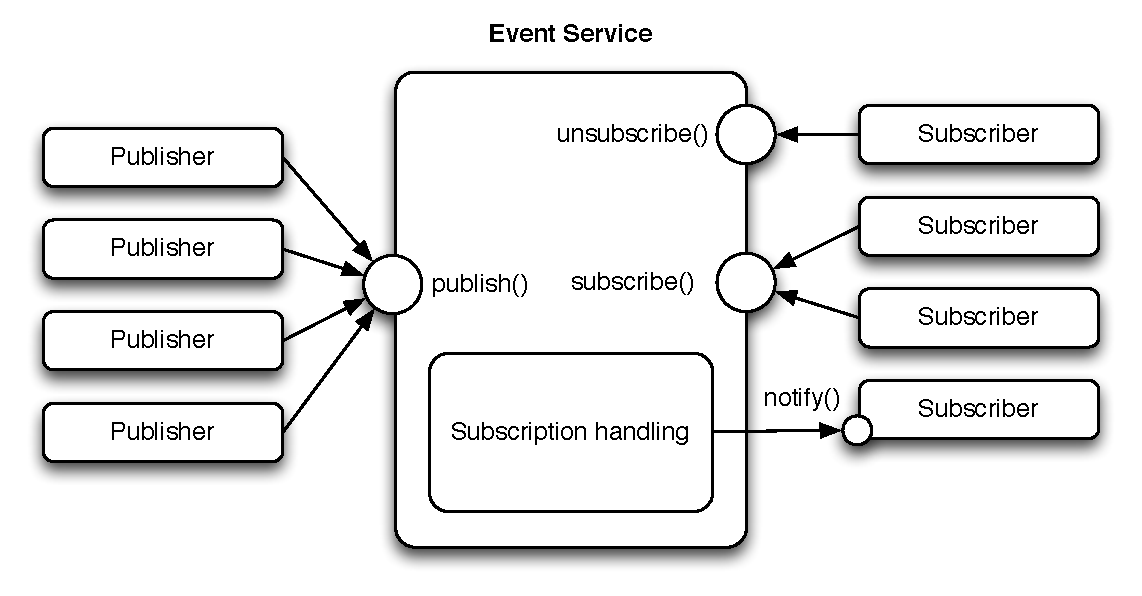
\includegraphics[width=\textwidth]{figures/pubsubarch}
\caption{The basic architecture of a pub/sub system.}
\label{fig:pubsubarch}
\end{figure}

The event service functions as an intermediary between publishers and
subscribers. It provides a level of indirection, as well as a service
interface. Publishers are able to generate new events through the
\texttt{publish} service call. It is now the responsibility of the event
service to determine which subscribers are interested in receiving this
event, and how to route the event to them. The subscribers register
their interest through a \texttt{subscribe} service call. The event
service will then store each subscribers interest in order to
disseminate events correctly. The publishers are then able to cancel
their subscriptions through a \texttt{unsubscribe} service call. No
information is forwarded from subscribers to publishers or from
publishers to subscribers.

The pub/sub paradigm provides a higher degree of decoupling than other
traditional approaches, in general, there are three types of decoupling
such a system provides:

\begin{enumerate}
    \item Space decoupling
    \item Time decoupling
    \item Synchronization decoupling
\end{enumerate}

Space decoupling means there are no need for the publisher and
subscribers to be know about each other. Subscriptions are handled by a
third party. Time decoupling assures that events are delivered
regardless of whether or not publishers and subscribers are online at
the same time, while synchronization decoupling refers to the fact that
neither publishers or subscribers are blocked when attempting to perform
their operations. While many other approaches can provide the first two forms of
decoupling, the main advantage of pub/sub is its fully asynchronous nature.
Approaches such as tuple spaces or message queues cannot completely
provide this synchronous decoupling, as messages are retrieved in a
synchronous manner. This property is key to the suitability for pub/sub
in large distributed system.~\cite{Eugster:2003}

\subsection{Message Filtering in Pub/Sub}

The subscription semantics of the pub/sub paradigm plays an important
role in the performance and flexibility of the system as event messages
are routed and managed based on topic or content. There are three
distinct types of subscription schemes:

\begin{enumerate}
    \item Topic-based
    \item Type-based
    \item Content-based
\end{enumerate}

In Topic-based systems, events are split into topics which are usually
represented as a string. In Type-based systems, events are filtered
according to the structure of the data, which provides type safety at
compile time. The  Content-based approach filters events based on a
global list of universal event attributes. This approach provides better
expressiveness in terms of filtering out the relevant events, however,
it also introduces more overhead with regards to handling
subscriptions. The complex filtering algorithms in content-based
approaches limit the scalability of
such systems with regards to the number of subscriptions. Type-based
share some similarities with content-based in the sense that the public members of the
types together form a description of the content of the event. Although
this ties the implementation of the pub/sub system closer to the
programming language, it still suffers from the same drawbacks as
content-based.

Topic-based offer less expressiveness than the other two subscription
schemes, but better performance if the set of possible event properties
is limited. Also, topic-based is more suited for dissemination and
multicasting, as topics can be thought of as groups, where subscribing
to topic T can be equivalent to joining the group for that topic. This
is a common approach taken by several proposed pub/sub
systems~\cite{Setty:2012, Castro:2002, Rahimian:2011, Wong:2008,
    Girdzijauskas:2010}

Traditionally, reliable multicasting of data through deterministic
dissemination has been the common approach. However, more recent
implementations investigate the potentials of probabilistic protocols,
which are more suited to the nature of decentralized systems and P2P.
These protocols do not guarantee full reliability of delivery, but provides a high
quantifiable \emph{probability} that events are delivered to all
subscribers.

\section{The Gephi Open Graph Viz Platform}

\begin{figure}[h]
    \centering
    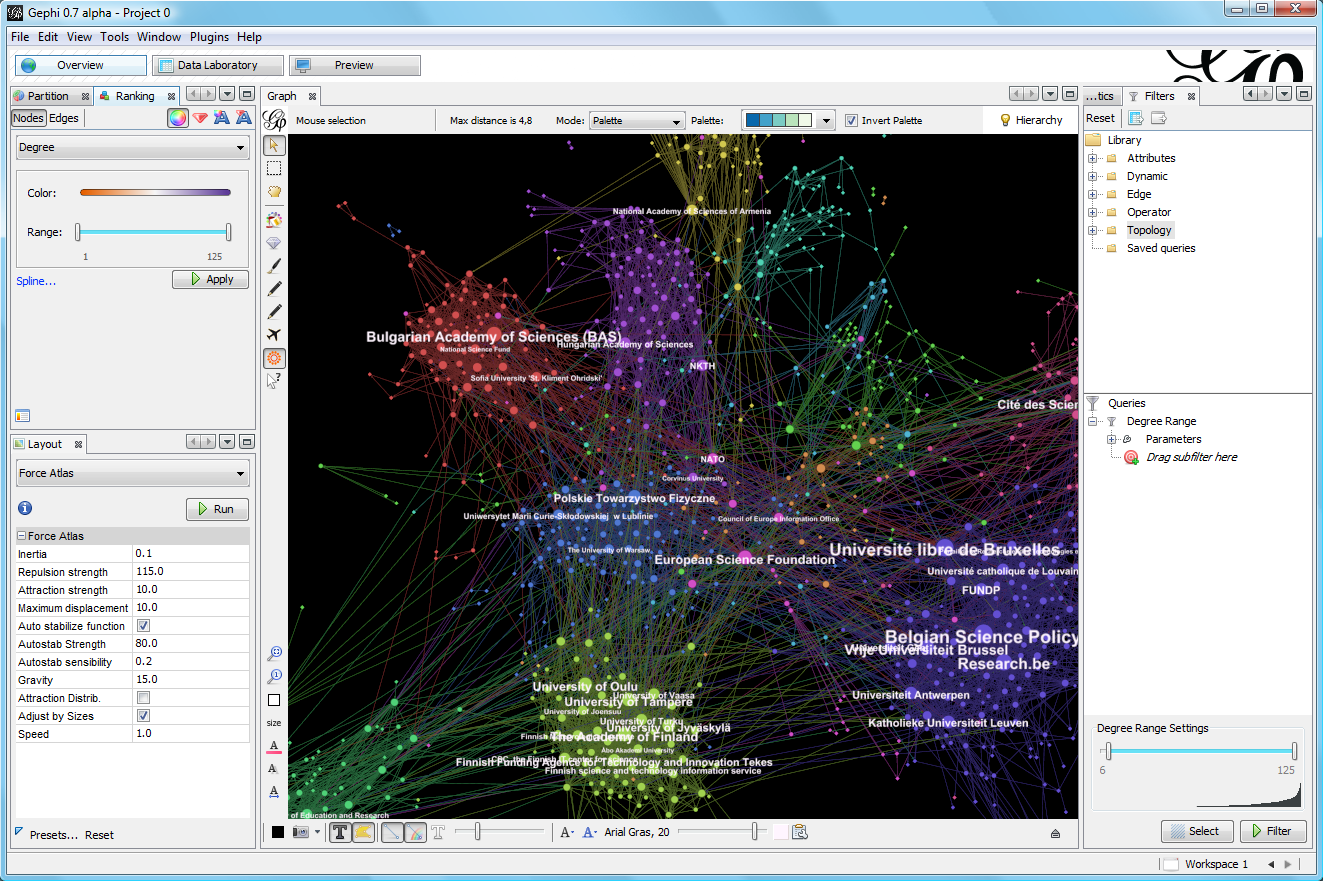
\includegraphics[width=\textwidth]{img/gephi1}
    \caption{The Gephi Tool supports
        visualization of graphs through coloring and sizing the visual
        graph
        representation. It also enables adding labels to nodes and
        edges. In
        this screenshot, Gephi is used to detect and visualize
    communities.}
\label{img:gephi1}
\end{figure}

Gephi~\cite{ICWSM09154} is an open source tool for exploring and
visualizing all kinds of networks, including dynamic and hierarchical
graphs. Described by the authors as ``photoshop for graphs'', Gephi
enables the user to interact with the graph structure, as well as
manipulate the colors and sizes of the visual graph representation in
order to display graph properties in an intuitive way. Gephi aims to
help researchers and data analysts in discovering patterns and revealing
hidden properties of the graph in question, as well as easily
discovering errors in the dataset. Gephi also provides a set of
statistical tools for measuring common metrics for Social Network
Analysis~(SNA) such as centrality, as well as metrics useful for general
graph topology analysis such as degree, path length and clustering
coefficient. Gephi is also useful in the emerging field of Dynamic
Network Analysis~(DNA)  as it supports temporal graphs, giving the user
the ability to filter the graph model according to a defined time
interval. It also support playback of the graph evolution, as well as
visualizing changes to graph data over time through size, color and text
labels which can be applied to both nodes and edges.

We consider tools such as Gephi to be a valuable addition to the field
of distributed systems research. Visual exploration of a dynamic network graph
is a useful approach to evaluation and development of such systems, as
some bugs are more easily spotted visually. For example, during our
implementation work, it was trivial to visually confirm that some edges
were missing from the graph visualization, leading to the discovery of a critical bug
in the implementation code which would otherwise be difficult to spot.
It is also worth to note that the different actors involved in the Gephi
project has formed a legal entity in the form of The Gephi
Consortium~\cite{gephi-consortium} in order to assure future development
of this tool. This, along with the fact that there seems to be a growing
community around this tool, gives us a certain degree of confidence that
this tool is something well worth investing in, as the risk of it
being discontinued or abandoned in the near future seems unlikely.

\section{The Gephi Toolkit}

In addition to the GUI-client, the authors of Gephi also provide an API
through the Gephi Toolkit project. The toolkit packages essential
modules from the GUI-client into a standard Java library which can
be used by any stand-alone Java project by including it as a dependency.
We take advantage of this toolkit in our implementation work, where it
is mainly used to handle and store information collected from PeerNet
simulations.

\section{The GEXF File format}

\begin{figure}[h]
\lstinputlisting[language=XML, label=lst:gexf-basic, frame=single]{listings/basic.gexf}
\caption{A GEXF description of a minimal static graph}
\end{figure}

The GEXF (Graph Exchange XML Format) file format~\cite{gexf} is an
effort by the Gephi Consortium to define a standard language describing
complex network structures. Being developed by the same authors,
the Gephi Tool is naturally fully compatible with this format, and is
able to both import and export GEXF files. This is also the case with
the Gephi Toolkit, as the module for handling such imports and exports
are included in this toolkit.

The GEXF file format is able to describe a graph through its nodes and
edges, as well as any data and dynamics associated with the graph. More
specifically, the file format is able to describe node, edges and their
associated attributes. Listing~\ref{lst:gexf-basic} provides an example
of a minimal static GEXF file, describing nodes, edges and attributes of
a graph.

\subsection{Dynamics}

\begin{figure}[h]
\lstinputlisting[language=XML, caption={}, label=lst:gexf-dynamics,
frame=single] {listings/dynamics.gexf}
\caption{Example of  dynamic GEXF file using spells}
\end{figure}

One of the major advantages of this file format is its support for
dynamic functionalities.  Both nodes, edges and attributes may have a
defined time interval where they exist. These lifetime intervals are
described as \emph{spells} if applied to nodes and edges, and as start
and end XML-attributes if applied to node or edge attributes. The
GEXF file in Listing~\ref{lst:gexf-dynamics} shows an example of a
dynamic graph where spells are used in order to determine the lifetime
of the nodes. The start and end times are by default encoded as
floating point values, however, dates are also supported, as seen in this example.

The support for dynamic graphs makes this file format an interesting
option for storing simulation data, and in our implementation work we
use this format extensively as part of our research effort.


\section{Pub/Sub Protocols} We create visualizations and evaluate the
performance for two different pub/sub protocols, namely
PolderCast~\cite{Setty:2012} and Scribe~\cite{Voulgaris:2005}. Both
protocols provide a message dissemination scheme, where nodes are
organized in a structured overlay. We briefly describe the relevant
details regarding each protocol, as we later will provide visualizations
of both the structure of these systems as well as their dissemination
scheme.

\subsection{PolderCast}

\begin{figure}[h]
    \centering
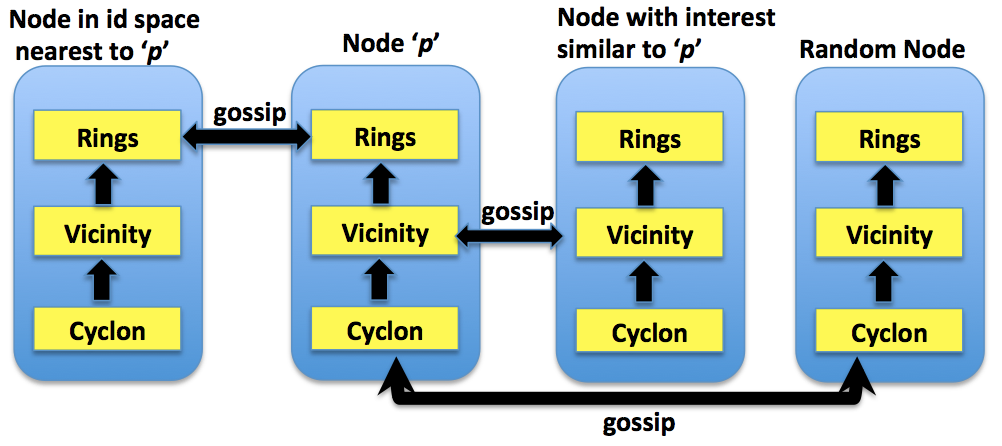
\includegraphics[scale=0.4]{img/poldercast_arch.png}
\caption{PolderCast consists of several decoupled components where a
    dissemination overlay is constructed at the RINGS layer}
\end{figure}

PolderCast~\cite{Setty:2012} is a topic-based
P2P pub/sub system which organizes nodes in a ring structure. The system
architecture of PolderCast is highly modular, and includes three
separate layers of overlay-based protocols. The CYCLON peer sampling
service~\cite{Voulgaris:2005} is used in order to maintain connectivity
across the whole set of subscribers, as well as providing the rings
layer with uniform random links. The Vicinity module consist of the
generic VICINITY protocol, which let nodes find neighbors based on a
\emph{proximity function}. This enables the construction of a RINGS
where neighbors of nodes participating in the ring are based on the
unique id of nodes, resulting in a ring sorted by node id. All the
protocol modules rely on gossiping for structural maintenance. This
means that at periodic intervals, a node $p$ will pair up with a
neighbor $q$ and exchange information regarding neighbors and
subscriptions.


\begin{figure}[h]
    \centering
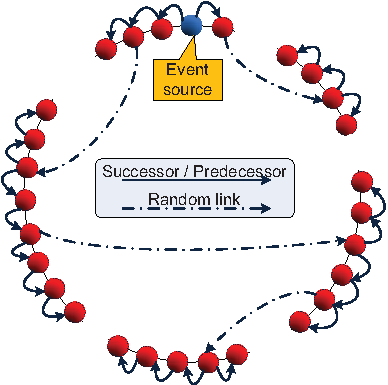
\includegraphics{img/hybrid_dissemination.pdf}
\caption{PolderCast utilizes a hybrid dissemination scheme when
    publishing messages, relying both on ring links as well as random
    links}
\end{figure}

% \begin{figure}
% 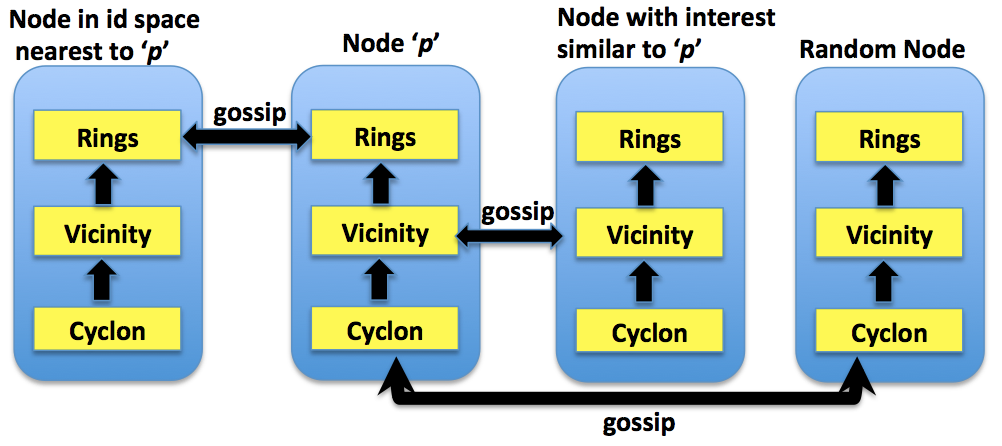
\includegraphics[width=\textwidth]{img/poldercast_arch.png}
% \caption{The system architecture of PolderCast is highly modular, each
%     layer has separate responsibilities and gossiping happens at every
%     layer}
% \end{figure}

PolderCast include a hybrid publication scheme using both
ring neighbors and random links in order to boost
dissemination, as well as increase resistance to ring
partitions and churn. The dissemination algorithm is based
on a configurable fanout $f$, and can be summarized in the
following steps for each node:

\begin{enumerate}
    \item If the message has already been received, discard it.
    \item If the message was received from a ring neighbor, forward it
        to the other ring neighbor, as well as to $f-1$ random
        neighbors.
    \item if the message was received from a random neighbor,
        forward it to both ring neighbors as well as to $f-2$ random
        neighbors
\end{enumerate}

\clearpage
\subsection{Scribe}

\begin{figure*}
    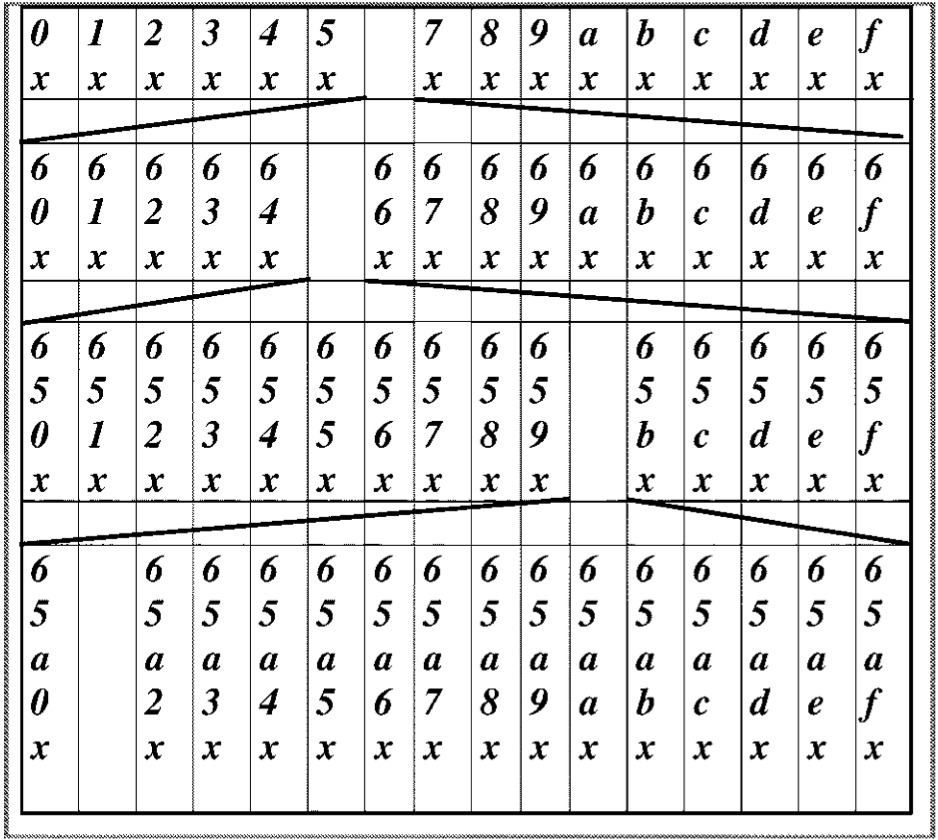
\includegraphics[scale=0.19]{img/pastry_table.png}
    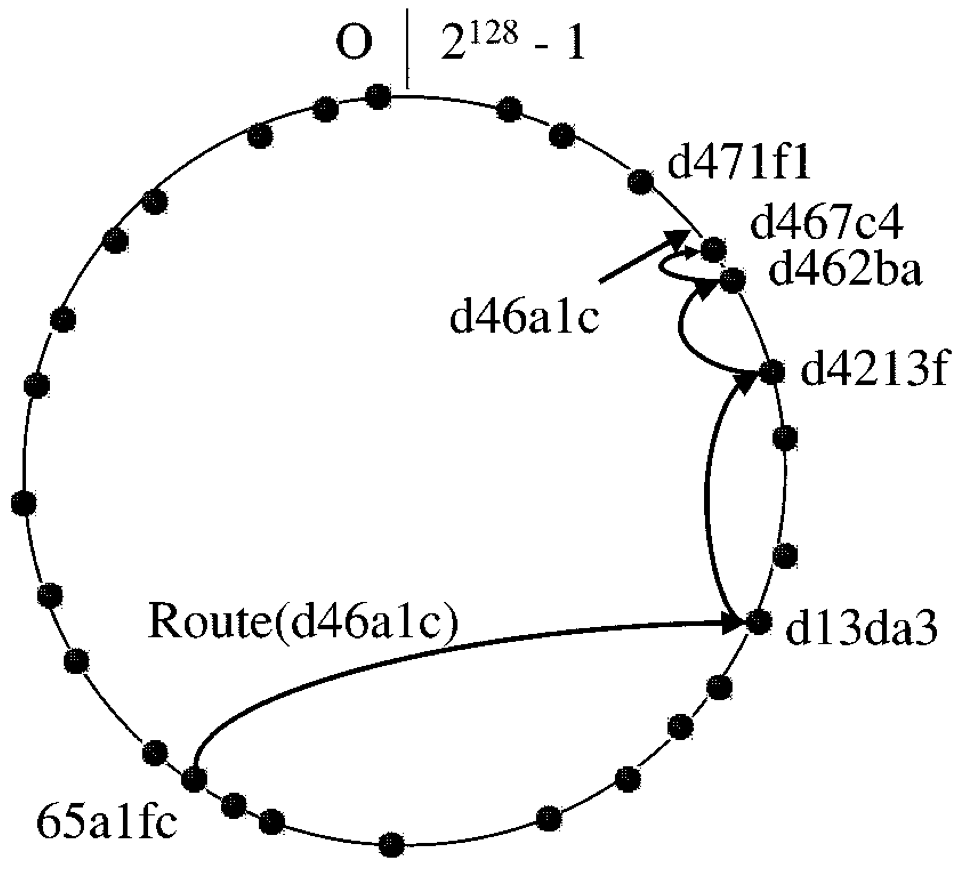
\includegraphics[scale=0.19]{img/pastry_routing.png}
    \caption{From
        left to right, the structure of a routing table in Pastry and an
        example of the Pastry routing scheme, where a message from node
        \emph{65a1fc} with key \emph{d46a1c} is delivered to the rendezvous
        node (figures borrowed from~\cite{Castro:2002})}
\end{figure*}

Scribe~\cite{Castro:2002} builds a dissemination overlay on top of
Pastry~\cite{Rowstron:2001}, a distributed hash table (DHT) which provides other
protocols with routing capabilities through an API\@. Scribe leverages
these capabilities in order to provide group and membership management
as well as message dissemination.

In Scribe, a tree structure is constructed for each group (i.e.\ topic).
These structures are maintained by having nodes send heartbeat
messages to its parent periodically. If a node suspects its parent is
dead, it will use Pastry to find a new parent.  When a node wants to
publish a message, it sends the publication to the root node of the
dissemination tree for that particular topic. This node is referred to as
a \emph{rendezvous node}, and is responsible for disseminating the
publication to its children. The initial phase of the dissemination,
where the message is routed to the rendezvous node, is handled by
Pastry. Pastry uses a routing scheme based on unique node ids living in
a circular namespace. Each node maintains a routing table of such ids,
where each row $n$ contains a sequence that match the id of the current
node in the $n$ first digits. When a node performs a lookup in the
routing table, it will traverse the table like a tree. It will start by
iterating through the entries in the first row until it finds a id
sequence which matches the key on the very first digit, then it will
lookup the row where the node ids all start with this digit, and iterate
through the entries until it finds the sequence which is a match on both
the first and the second digit. This will continue until an entry is
found which shares a prefix with the lookup key which is longer than the
current node id. If no such id is found, it will find an entry with a
prefix with the same size as the current node id, but where the
following digit is closer to the key. When the publication reaches the
rendezvous node, this node will continue the dissemination by forwarding
the publication to its children.

\section{The PeerNet Simulator}
PeerNet is an extended version of the
popular \emph{PeerSim simulator}~\cite{p2p09-peersim}. More
specifically, PeerNet adds a distributed simulation mode, where each
node, or a subset of nodes, can be executed in separate processes. This
means that unlike PeerSim, where execution of the protocols are
performed sequentially, each node in PeerNet is able to execute
in parallel. Also, in contrast with PeerSim, the execution of the
system happens in real-time. The higher degree of parallelism and
the real-time execution are two important factors which enable PeerNet to
provide a more realistic environment for running experiments. It is also
worth to mention that running in distributed mode is beneficial with
regard to scalability in terms of number of nodes included in the
simulation, as the memory and computational resources required to run
the simulation can be distributed across several machines. This is an
important factor as PeerNet is implemented in Java, which is a fairly
memory intense language when dealing with large-scale systems.

While PeerNet is able to extend PeerSim with a distributed mode, it also
provides a simulation mode which behaves exactly like simulations in
PeerSim, where experiments are run locally in one single process. In our
evaluation, we take advantage of both simulation modes in PeerNet. We
update existing PeerSim implementations of PolderCast and Scribe for use
with PeerNet, as well as implement a \emph{reporter interface} for these
protocols in order to make them compatible with our tool for visualizing
and evaluating such systems.

\section{Description of important metrics}

In the following section, we describe some of the metrics visualized and
analyzed in the following chapters. In general, the most common metrics
important for performance in pub/sub can be divided in three categories:
(1) structural overlay properties, (2) dissemination properties and (3)
communication overhead due to overlay maintenance.

\subsection{Structural overlay properties}
\begin{description}
\item[Node Degree]\hfill\\

The degree of a node is determined by the number of connection to its
neighbors. Degree can both be undirected and directed. Directed degree
separates between in-degree and out-degree, where the former is a
measure of the number of connection to this nodes from neighbors, while
the latter is the number of outgoing connections from the particular
node. A skewed distribution of directed edges would reveal an imbalance
in the constructed overlay, or reveal vulnerable points in the system.
Also, it is essential to understand how the system scales with regard to
the number of topics a node is interested in. For example, if the number
of edges increases linearly with the subscription size of a node,
scalability suffers. A poor degree distribution affects load balancing,
high degree nodes have an increased likelihood of being overloaded, and
might introduce bottlenecks in the system.

\item[Topic diameter]\hfill\\

This metric is a measure of the maximum number of hops between any two nodes that
share interests, i.e.\ a measure of the diameter of a subgraph
consisting only of nodes who registered their interest in the
same topic. Having a low topic diameter is beneficial for
disseminating events on a topic.

\item[Clustering coefficient]\hfill\\

This is the ratio of number of edges between neighbours of a node $n$
over the total number of possible edges between them. In simpler terms,
how many of a nodes neighbours are connected to each other. A high
clustering coefficient would indicate that the network has a higher risk
of partitioning, as well as a risk of having a higher number of
redundant message deliveries.

\item[Betweenness centrality]\hfill\\

Betweenness is the number of times a particular node is found on the
shortest path between two other nodes. A node with a big betweenness
centrality may constitute both a vulnerable part of the graph as well as
a bottleneck, as it might take part in a high number of event
disseminations.

\item[Closeness centrality]\hfill\\

Closeness is a measure of how close the particular node is from
every other node in the network. More specifically, it is the
average distance in terms of shortest path length to every other
node in the graph. Closeness is typically regarded as a measure of
how long it will take to disseminate data from a node $n$ to every
other node in the network sequentially~\cite{newman2005measure}.

\item[Eccentricity centrality]\hfill\\

Eccentricity measures how far away a node $n$ is from the node most
distant from it in terms of path length. The maximum eccentricity is is
the Graph Diameter, i.e.\ the longest path between any two nodes in the
graph.

\end{description}

\subsection{Dissemination properties}

\begin{description}

\item[Hit-ratio during churn]\hfill\\

Hit-ratio is the fraction of subscribers that received a publication message, over
the total number of subscribers for that topic. It is essential to
understand how the different systems respond to churn when disseminating
events i.e.\ how the system deals with nodes both leaving and joining
the network. If an overlay is robust, it should provide a high hit-ratio in
the presence of realistic churn. Meaning that at very high percentage
of subscribers receive the appropriate events.

\item[Path Lengths]\hfill\\

Dissemination path lengths is the number of nodes a publication message
traverses before reaching its target subscriber i.e.\ the \emph{number
of hops} the publication messages makes from node to node. This
metric is helpful in order to understand the efficiency of the
dissemination algorithm.

\item[Number of duplicate messages]\hfill\\

Subscribers might receive the same publication message several times,
depending on the method of dissemination being used. Epidemic
dissemination schemes usually infer a higher number of duplicate
messages. Redundant messaging incurs a overhead cost in terms of
bandwidth as well as processing power at the receiving node.

\end{description}

\subsection{Maintenance overhead}

\begin{description}
\item[Number of control messages]\hfill\\

Some systems rely on control messages in order to maintain the overlay
topology. For example in Scribe, where the multicast tree structures are
maintained with periodic heartbeat messages. The number of control
messages a node sends and receives serve as an indicator of this
overhead.

\item[Control message bandwidth consumption]\hfill\\

Control messages also constitute overhead in terms of bandwidth usage.
Measuring the control message overhead in terms of number of bits sent
and received from each node reveals the bandwidth cost, revealing any
potential bottlenecks or overloaded nodes.

\end{description}
